\section{Feature Importance}
\label{sec:feature-importance}

One way to determine the importance of a feature for a model is called 
permutation feature importance. Here, the model is trained like usual but during the prediction step, 
we use a modified version of the test data where one feature is randomly permuted over all forecast cases. 
This way, the model cannot use the information of this feature properly 
and will most likely perform worse. The loss on the shuffled dataset is 
then divided by the loss on the regular test set. A value close to \(1\) 
indicates that the feature is not that important because the model doesn't perform 
much worse than before. The higher the quotient, the more important the feature is for the model.
Since our time series heavily depends on the time of day, it makes sense 
not to shuffle the whole feature but only the equivalence classes of each hour, 
i.e., the values at \(1\) AM are shuffled, the values at \(2\) AM are shuffled, etc.

Figure \ref{fig:feature-importance} 
shows the results of the permutation feature importance calculation. 
We can see that the feature importance value for surface solar radiation downwards 
is highest for QRF and NNQF while the total cloud cover predictor is the most important 
for SQF-RNN.

\begin{figure}[h!]
    \begin{tikzpicture}
    \begin{axis}[
        width  = \textwidth,
        height = 0.3\textheight,
        major x tick style = transparent,
        ybar,
        bar width=10pt,
        ymajorgrids = true,
        ylabel = {Feature importance},
        xtick = {1,2,3,4,5,6},
        xticklabel style={align=center},
        xticklabels = {Surface\\solar\\rad down, Surface\\thermal\\rad down, Top net\\solar rad, Total\\precipitation, Total\\cloud cover, Previous\\points},
        scaled y ticks = false,
    ]
        \addplot
            coordinates {(1, 1.3365) (2, 1.0214) (3, 1.0199) (4, 1.0020) (5, 1.0025)};
        \addplot
            coordinates {(1, 1.2202) (2, 1.0052) (3, 1.0856) (4, 1.0032) (5, 1.0405)};
        \addplot
            coordinates {(1, 1.0268) (2, 1.0208) (3, 1.0516) (4, 1.0124) (5, 1.2059) (6, 1.0918)};

        \legend{QRF, NNQF, SQF-RNN}
    \end{axis}
\end{tikzpicture}
    \caption[Feature importance]{Feature importance. 
    The table shows the permutation feature importance quotients. 
    The permutation feature importance quotient is 
    the loss of the model with shuffled feature 
    divided by the loss of the model without shuffled feature. 
    A higher value indicates a more important feature.
    Since only the SQF-RNN model uses the previous points for the prediction, 
    we can only calculate the feature importance of the previous points for this model.}
    \label{fig:feature-importance}
\end{figure}